\chapter{吞咽困难}

正常吞咽功能发生障碍时称为吞咽困难,患者在咽下食物时有梗阻的感觉,并常能指出梗阻的部位。其主要原因是:①食管的机械性梗阻。②支配吞咽功能的神经肌肉发生病变或功能失常。③口腔、咽、喉等处的疼痛性或梗阻性病变。

吞咽困难的病变部位可分为三类:

\section{1.口腔、咽、喉与上段食管病变}

例如口、舌的疼痛性或梗阻性病变,干扰正常的吞咽动作。各种原因如重症肌无力、白喉等所致的咽麻痹,也可引起吞咽困难。

\section{2.食管中段的病变}

吞咽后2~5秒钟发生的吞咽困难,应注意中段食管的病变。此外,胸部主动脉瘤、纵隔炎、纵隔淋巴结结核与赘生物、肺脓肿也应考虑。显著的心脏增大、心包炎、胸膜炎、脓胸偶尔也可压迫中段食管而引起吞咽困难。

\section{3.食管下端数厘米部位的病变}

在吞咽后5~15秒钟发生的剑突后部位不适感、疼痛或阻塞感,提示病变在下段食管。

患者取坐位,将听诊器放置于其剑突的左侧,嘱患者饮水一口,如无食管梗阻,则约于10秒钟之内可听到喷射性杂音。食管梗阻(如食管癌、贲门失弛缓症、食管良性狭窄等)时,此杂音延迟出现或不明显。体检对由神经病变、骨骼肌和咽部疾病引起的吞咽困难有重要意义。除全身性神经肌肉病证据外,应注意有无球麻痹(延髓麻痹)或假性球麻痹体征,如构语障碍、发音困难、上睑下垂、舌萎缩或颌反射亢进。

吞咽困难这一症状往往有重要的临床意义。但吞咽困难应与涉及吞咽的一些其他症状相鉴别,如癔球症、癔症。癔球症在不进食时也感到咽喉或胸骨后有一块上下移动的物体堵塞,但实际吞咽通畅,并无困难,多见于女性,与情绪因素有关,客观检查并无梗阻发现;而癔症常表现恐食症,患者吞咽恐惧,拒绝进食。成人的食管腔由于管壁有弹性可扩张至4cm,若扩张达不到2.5cm就可出现吞咽困难症状,如达不到1.3cm必有吞咽困难。食管壁病变引起管腔周径狭窄者,要比食管偏心性狭窄更易引起吞咽困难。出生后或哺乳期即出现间歇性或经常性食后呕吐或吞咽困难,应考虑食管先天性疾病。儿童突然出现吞咽困难常由于食管异物阻塞。吞咽困难伴有食物经鼻腔流出,提示主管吞咽活动的神经肌肉发生病变,如咽麻痹。吞咽时伴有咕噜声提示Zenker憩室存在,吞咽困难伴胸痛常发生在弥漫性食管痉挛以及因食团大而引起的急性吞咽不能,吞咽困难伴声嘶,提示肿瘤压迫喉返神经。贲门失弛缓症时,食物反流量往往较食管癌时多,而食管癌时可能混有血液,并呈进行性吞咽困难。反流性食管炎时,吞咽困难常伴有胸骨后或心窝部烧灼痛,饱餐后仰卧位疼痛发作或加剧。吞咽困难发生于中年以上,病程短,全身情况差,多考虑癌性梗阻。发病于青壮年,病程长,全身情况良好,常为良性梗阻。

食管钡餐X线检查与胃镜检查是诊断食管疾病不可缺少的手段,尤其对于良性与癌性食管梗阻的鉴别诊断有重要意义。脱落细胞学检查和食管动力学检查,食管pH监测和食管多通道腔内阻抗-pH监测以及胸部X线片、超声内镜及CT检查也能很好地帮助查找病因。

引起吞咽困难的疾病颇多,现按表\ref{tab19-1}顺序讨论如下。

\begin{table}[htbp]
\centering
\caption{吞咽困难疾病的分类}
\label{tab19-1}
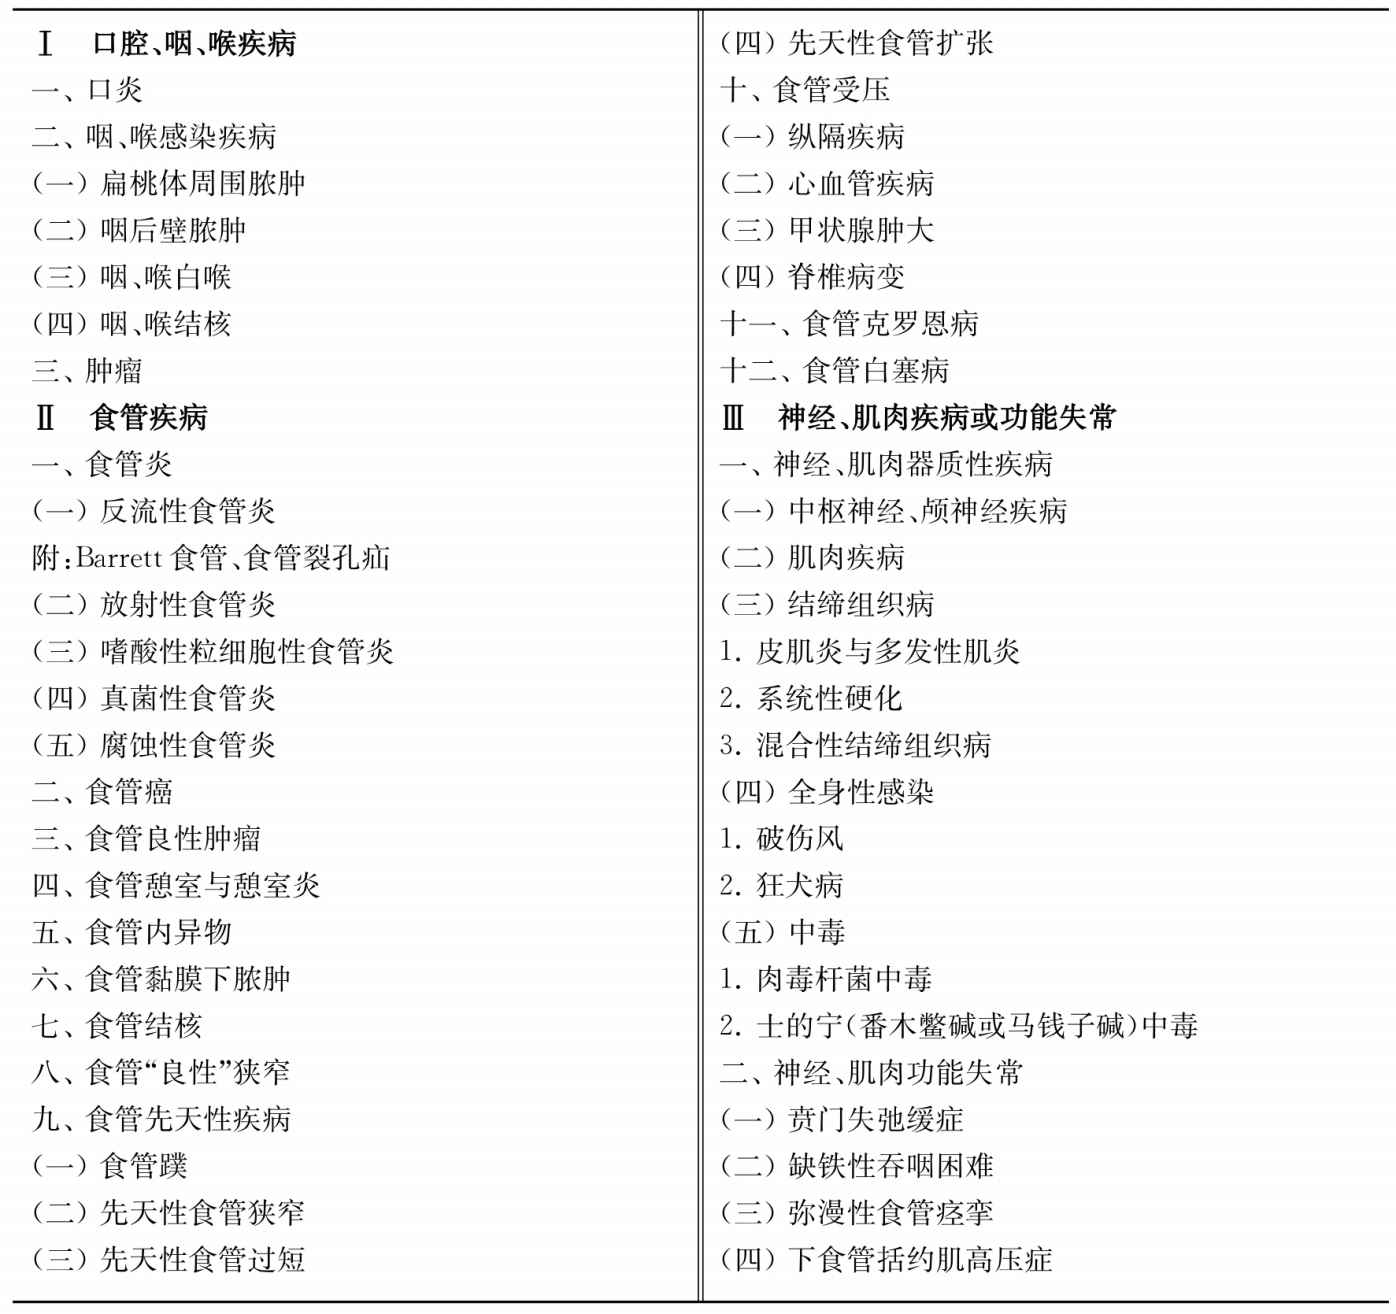
\includegraphics[width=5.90625in,height=5.55208in]{./images/Image00119.jpg}
\end{table}

\protect\hypertarget{text00155.html}{}{}

\section{60 口腔、咽、喉疾病}

\subsection{一、口 炎}

各种原因的口炎,如伴有剧烈的疼痛患者拒绝吞咽都可引起吞咽困难。干燥综合征由于唾液分泌减少也可引起吞咽困难。

\subsection{二、咽、喉感染疾病}

咽部的疼痛性与梗阻性病变,可引起吞咽困难。最明显的是扁桃体周围脓肿与咽后壁脓肿。

\subsubsection{(一)扁桃体周围脓肿}

扁桃体周围脓肿是腭扁桃体周围组织的化脓性炎症,常于急性扁桃体炎病程第三、四天左右发生。发病多在15~35岁之间。病变大多为单侧性。致病菌通常为溶血性链球菌与葡萄球菌。患者以恶寒、发热、不适感、头痛、咽痛、纳差等症状起病。血象中性粒细胞增多与左移。咽痛逐渐加重,常向患侧耳部放射。

患者张口与吞咽均感疼痛与困难。饮水时水常向鼻腔反流。病侧颈淋巴结肿痛。咽部检查可见扁桃体充血肿胀,其表面往往有渗出物。腭垂向对侧推移,发音时软腭运动异常,常带有鼻音。扁桃体周围脓肿应及时应用抗感染药物治疗与切开排脓。

\subsubsection{(二)咽后壁脓肿}

咽后间隙充填以疏松结缔组织,婴儿时期含有淋巴结8~10个,至3~8岁逐渐消失。咽后壁脓肿的原发感染常为上呼吸道病灶,经淋巴道传播而引起此病。患者以周岁以内婴儿最多,成人患病较少。在化脓性中耳炎时,细菌可经淋巴道感染而引起咽后壁脓肿。咽后壁异物损伤也可为脓肿形成的诱因。病儿常以恶寒、发热、不适、纳差、烦躁不安等全身症状起病。脓肿形成后即可发生不同程度的吞咽与呼吸困难。病儿常将头部偏向一侧以减轻呼吸困难与疼痛。颌下与颈淋巴结常肿痛。

咽后壁高度充血与不同程度的肿胀。咽后壁脓肿是一严重的疾病,脓肿突然破溃可引起窒息(故做咽后壁检查要做好急救准备);如向附近组织蔓延可引起广泛性蜂窝织炎;如吸入气管可引起肺部化脓性疾病;细菌进入血内可引起败血症。

\subsubsection{(三)咽、喉白喉}

咽、喉白喉可引起疼痛与吞咽困难,但一般不甚剧烈。

\subsubsection{(四)咽、喉结核}

咽、喉结核常继发于开放性肺结核。口咽部结核性溃疡可引起剧烈的疼痛与吞咽困难。溃疡甚浅,基底为灰白色的肉芽或坏死组织,边缘不整,呈凿缘样,周围黏膜无明显的炎症反应,患者并有咳嗽、潮热、盗汗、消瘦等症状以及肺结核的胸部体征。喉结核则以声音嘶哑为突出的症状,并可因喉痛而有吞咽疼痛、吞咽困难等症状。

\subsection{三、肿 瘤}

如口腔癌、舌癌、喉癌、鼻咽癌等。

\protect\hypertarget{text00156.html}{}{}

\section{61 食管疾病}

\subsection{一、食管炎}

\subsubsection{(一)反流性食管炎}

胃、十二指肠内容物反流入食管,引起烧心、反酸、胸痛等症状,称为胃食管反流病(GERD)。根据内镜检查是否存在食管炎而可分为内镜阴性的胃食管反流病(又称非糜烂性反流病,NERD)及反流性食管炎(RE)。胃食管反流病除了有食管表现以外,还可以有食管外表现,如咳嗽、哮喘、声嘶等。部分RE患者可有吞咽困难,可由于食管动力异常引起,少数由RE的并发症食管狭窄引起。由食管痉挛或运动紊乱所致的吞咽困难为固体和液体食物通过均困难,呈间歇性,且经常发生在开始进餐时。而食管狭窄的吞咽困难呈持续性,对干食尤为明显。内镜检查是确诊RE最准确的方法,并能判断严重程度及有无并发症,并排除其他食管病变。对有典型烧心和反酸症状,结合内镜检查所见即可作出反流性食管炎的诊断。对症状不典型者,需结合内镜检查、24小时食管pH监测和质子泵抑制剂治疗试验进行综合分析以作出诊断。1994年第十届世界胃肠病会议提出了洛杉矶分级法:A级,一个或一个以上食管黏膜破损,长径<5mm;B级,黏膜破损>5mm,黏膜破损无融合;C级,黏膜破损融合,但<75\%食管周径;D级,黏膜破损融合,至少达到75\%食管周径。反流性食管炎可并发食管溃疡、狭窄和Barrett食管。

Barrett食管(BE):是指食管鳞状上皮被化生的单层柱状上皮所取代,如发生溃疡称为Barrett溃疡。BE主要因长期的胃食管反流所致。BE本身不引起症状,患者的症状主要是由于RE及其并发症所致。Barrett食管患者发生食管腺癌的危险性大大高于自然人群。BE诊断最可靠的方法是内镜下活检行病理检查。内镜下可发现食管下端有橘红色黏膜,常呈三种类型:①岛型;②环周型;③舌型。如识别困难,可从内镜活检孔向可疑区域喷洒卢戈碘液,鳞状上皮着棕色,而柱状上皮不着色。

食管裂孔疝:食管裂孔疝是指胃的一部分通过横膈食管裂孔进入胸腔。本病发病率随年龄增加,其中以滑动型最多,约占食管裂孔疝的90\%,其他还有食管旁裂孔疝及混合型食管裂孔疝。食管裂孔疝可以无症状,可以不伴发RE,而有食管裂孔疝的RE症状及食管炎症常较重。X线钡餐检查是诊断本病的主要方法,可有以下表现:①膈上疝囊征;②膈上食管胃环征;③疝囊内胃黏膜皱襞影;④膈食管裂孔增宽,>2cm。内镜检查可发现齿状线上移、贲门口松弛增宽,可见胃囊进入食管腔。

\subsubsection{(二)放射性食管炎}

因食管癌、纵隔肿瘤而接受放疗的患者,几乎均可发生放射性食管炎。放疗1~2周后可出现食管黏膜充血、水肿,患者出现吞咽疼痛,胸骨后不适及吞咽困难等症状。如放疗反复持续4~8个月,可出现食管慢性损害,如食管溃疡、狭窄和瘘管,患者表现为进行性吞咽困难,皮质激素可用于治疗放射性食管炎。

\subsubsection{(三)嗜酸性粒细胞性食管炎}

嗜酸性粒细胞性食管炎(eosinophilic
esophagitis,EOE)是一种免疫抗原介导的慢性食管疾病,其组织学上表现为食管黏膜嗜酸性粒细胞(EOS)浸润为主的炎症变化,临床上表现为食管功能障碍相关症状,如吞咽困难、食物嵌顿、呕吐、上腹痛等。近年国外对EOE报道日益增多,国内较少。该病可发生于各个年龄段,青少年和儿童好发。

50\%患者有过敏体质病史,如鼻炎、食物过敏、特应性皮炎、支气管哮喘等。临床表现多样,易与GERD混淆。为了排除GERD,可给予6~8周PPI治疗,或行24小时食管pH监测,EOE对抑酸剂不敏感且24小时pH正常。食管压力测定表明EOE有动力障碍,但并非EOE所特有。EOE内镜下表现无特异性,主要为:线状沟槽、黏膜粗大水肿、食管狭窄;EUS可发现黏膜肌层呈环形但不对称增厚。研究显示24.8\%EOE患者因内镜下黏膜无变化而漏诊,因此对有吞咽困难或食物嵌顿患者,即使内镜下未发现异常变化,亦建议行组织病理学检查。建议于上端、下段及病变处食管黏膜总共取6块组织活检(其诊断敏感性达100\%),同时取胃和十二指肠黏膜活检以排除该部位病变。

X线检查并非诊断EOE的主要方法,其表现正常亦不能排除EOE,但是食管X线及CT检查可发现食管解剖学畸形,亦可提供食管狭窄及管壁增厚情况,有助于判断是否需行食管扩张术。2011年EOE共识提出的诊断标准:①临床症状:食管功能障碍相关症状;②组织病理学改变:食管黏膜EOS计数≥15个/HPF;③排除GERD及其他可引起EOS浸润的疾病。对部分食管EOS数目达到EOE标准,但对PPI治疗有效称为PPIRee(PPI-responsive
esophageal
eosinophilia)。但之后即使维持PPI治疗,也会反弹,因此认为其是早期的EOE,是EOE亚型,因此在长期PPI单独治疗过程中应监测EOE以减少漏诊。但PPIRee是EOE亚型或GERD亚型或自成一类疾病目前尚不明确。

\subsubsection{(四)真菌性食管炎}

重症糖尿病、鹅口疮、长期用广谱抗菌素、免疫功能低下者、艾滋病易罹患本病。患者多以咽下困难、胸骨后疼痛、纳差为主诉。内镜检查典型表现为成片的黏膜上皮被覆乳白色或绿色黏稠分泌物的假膜斑块,其下方为红斑状质脆黏膜。内镜直视下细胞刷刷取食管黏膜直接涂片镜检较易得到阳性发现而确定诊断。对无糖尿病、恶性肿瘤及口服激素、免疫抑制剂、肿瘤化疗患者,出现真菌食管炎,应注意排除艾滋病可能。

\subsubsection{(五)腐蚀性食管炎}

指误食吞服化学腐蚀剂造成食管严重损伤引起的炎症。腐蚀剂包括各种强酸、强碱、消毒水等,多见于误服或自杀者。吞入腐蚀剂后即引起口、咽、食管及胃黏膜烧伤而产生灼痛,发生反射性呕吐、吞咽困难。烧伤瘢痕可致食管狭窄。常用碘水口服代替吞钡造影,以观察食管病变及排除穿孔。

\subsection{二、食管癌}

食管癌的发病率在我国北方较高,男性发病显著高于女性。罹患年龄大多在50~70岁,而51~60岁发病率最高。发病部位以中、下段食管居多,各占食管癌的40\%以上。长期饮用烈酒,常食偏干、偏硬、偏热与强烈刺激性食物与食管癌发生有一定关系。此外亚硝胺化合物、营养不良和微量元素缺乏以及遗传因素均与食管癌有关。慢性长期反流性食管炎因为经常合并Barrett食管,后者发生食管腺癌危险性明显升高,近年西方国家食管腺癌发病率逐年升高与胃食管反流病发病率升高密切相关,但我国仍以食管鳞癌为主。食管癌早期无自觉症状,至癌逐渐增大,方出现症状。开始时仅为食物通过时有不适感,并不严重,进而出现吞咽困难。食物通过食管某一部位时有阻塞感,由间歇性变为经常性。初时不能进干食物,继而半流质甚至流质也不能进食。从症状开始出现至症状明显常需几周至几个月,甚至一年以上。其他常见症状是疼痛,一般于较晚期出现,患者咽下食物时觉胸骨后或背部疼痛。下段食管癌或贲门癌病者的疼痛与不适感常在心窝部,这种情况多见于溃疡型癌。贲门癌所致的吞咽阻塞感与吞咽困难出现较晚,发现时常已是晚期,往往失去治疗时机。因此对有吞咽不适患者,应及时做胃镜检查,对疑似患者应择时复查,直到明确诊断。食物反流、出血与体重减轻等是较晚期的症状。

在诊断方面,凡患者有反复出现的或进行性吞咽困难、吞咽梗阻感或不适感、吞咽时胸骨后或心窝部疼痛,尤其40岁以上的男性,应考虑食管癌的可能性,有干食、硬食、热食的习惯者尤须注意。下段食管癌的临床症状常与溃疡病相似,如有心窝部灼痛、不适感、反酸、嗳气、呃逆等,临床医生应有所警惕。X线钡剂食管造影可见局部黏膜中断、破坏,腔内充盈缺损或狭窄,管壁僵硬、蠕动消失,钡剂通过障碍。在癌阻塞的上方少见有食管扩张,但如为良性瘢痕性狭窄或贲门痉挛所致的狭窄,则狭窄部上方的食管常有高度扩张。

如X线检查发现食管下端狭窄而未发现食管癌的证据时,应作胃镜详细检查贲门胃底,排除贲门胃底部癌的可能性。并且应分段取病理,如为食管癌多为鳞癌,如为贲门胃底癌多为腺癌,但应注意有些食管癌可侵犯贲门胃底。超声胃镜及CT可协助诊断。临床上应特别注意,无吞咽困难并不能排除食管癌。

有些食管癌病例特别是早期病例,须经胃镜检查方能确定诊断。胃镜检查可达到直接观察癌和做活组织检查的目的,以进一步明确肿瘤的性质和分级,提供治疗上的参考,它是确定诊断的最好方法。镜下用卢戈碘或甲苯胺蓝染色有助于早期癌组织病变范围及内镜活检部位的确定。一次镜检结果为阴性,而临床上仍有可疑时,应于2~3周后复查。超声内镜对食管癌的鉴别诊断,TNM分期评估以及引导淋巴结穿刺有较大帮助。

近年国内应用摩擦气囊采取食管癌脱落细胞作涂片检查,早期癌发现率因而大大地提高。又应用食管分段拉网的方法进行早期癌定位,经过X线与手术切除标本证实是可靠的方法。这些方法已在我国农村和部分城市广泛应用,特别是在食管癌高发区进行普查时。

\subsection{三、食管良性肿瘤}

食管良性肿瘤少见,其中以食管平滑肌瘤占最多数,患者大都为男性,约半数发生于21~40岁之间。此瘤可生长在食管各段,大小不一,单发或多发,但单发最为常见,有的有蒂,有时可将肿瘤呕出。当肿瘤增大阻塞食管腔,才出现吞咽不适或疼痛等症状。

50\%以上的食管平滑肌瘤有不同程度的吞咽困难,多数轻微,或呈间歇性,甚少影响正常饮食。此外为疼痛(吞咽痛、胸骨后痛、背痛、心窝部痛)与消化不良症状(食物反流、食后不适、心窝部灼热感)。病程较长,有达十几年者,此点与食管癌有所不同。患者症状虽轻,但与X线食管钡剂造影所见的病变范围常不相称,此点与食管癌也有重要鉴别诊断意义。食管钡剂造影可见边缘清晰而光滑、呈半圆形的充盈缺损,缺损与正常食管有清晰的分界,两者之间常呈锐角,肿瘤部位黏膜皱襞消失,但无黏膜破坏与龛影。胃镜检查有助于诊断,特别是超声内镜可帮助诊断并判定肿瘤起源于哪一层,并指导内镜下治疗。其他食管良性肿瘤还有食管腺瘤、食管乳头状瘤、食管血管瘤、食管囊肿等,均较少见。

\subsection{四、食管憩室与憩室炎}

食管憩室可发生于食管任何部分,但最多发生于食管上端,其次为中段食管与膈上部食管。从病因与病理方面,食管憩室可区分为膨出型与牵引型两类。

咽食管憩室(Zenker憩室)是膨出型憩室,也是最常见的一种,发病在40~70岁之间,组织学上是由复层鳞状上皮和黏膜下层所组成,肌肉层只存在于憩室的颈部;憩室大小不一,直径可自2~3cm至5~10cm。初期无症状,或偶有咽部不适感或口涎增多。憩室逐渐增大时。患者进食时常觉有食物进入囊内,并有食物反流。饮水时可出现气过水声。如憩室被潴留的食物所扩大,则可压迫食管而引起吞咽困难,或致颈根部一侧有肿物膨出。症状可周期性出现,这是由于憩室逐渐被食物所充盈而达到可引起梗阻的程度,才引起症状。此时憩室可因呕吐而清除了内容物,因而出现一段缓解期。憩室可因食物潴留与刺激而继发炎症与溃疡,甚至发生出血与穿孔。

牵引型憩室常发生于食管中段,主要位于肺门相对的食管,大多数由于肺门淋巴结结核瘢痕性牵引所致,少数由于心包炎瘢痕性牵引所致。此型憩室一般无明显的症状,大多在胃肠钡餐检查时偶然发现,直径通常为1~2cm,一般为单个。如有炎症、水肿、痉挛或溃疡形成,可出现胸骨后痛、吞咽不适感甚至出血。

食管憩室的诊断主要依靠X线食管钡剂造影检查,在正、侧及斜位摄片上,可显示憩室的部位、大小以及与食管腔的关系。胃镜检查可发现憩室有无并发炎症与溃疡,应循腔缓慢插入内镜,以防止穿孔发生。

\subsection{五、食管内异物}

食管异物半数以上发生于10岁以下的儿童,以骨类、金属制品(如硬币)、果核、假牙等为最常见。大多数异物被卡住于颈部食管,多位于环咽肌的下方,即胸腔入口部,此处是食管最狭小部分。由于局部刺激或损伤所致的黏膜炎症水肿与肌肉痉挛,异物固定于此处而很难向下方移动。

食管异物都可引起不同程度的吞咽困难与吞咽痛。重症患者完全不能进食,轻症患者也只能食半流质。异物卡住于食管上端可压迫气管后壁而引起呼吸困难,儿童罹患尤为多见。儿童患者常有垂涎增多。有食入异物病史而垂涎增多,提示异物存在于颈部食管,而不在胸部食管。

X线检查可见不透X线的异物阴影,钡剂分流现象等。异物可经胃镜发现并取出。

\subsection{六、食管黏膜下脓肿}

食管黏膜下脓肿是罕见的食管疾病。各种原因所致的食管黏膜损伤是发病的基础,并因口腔、咽部致病菌的咽下而致感染。主要症状是吞咽困难与胸骨后痛,呈烧灼样痛,在咽下时加剧。患者常有发热、全身不适、乏力与食欲减退等全身症状。偶尔可引起大出血。X线食管钡剂造影可发现表面光滑、凸出的充盈缺损。胃镜检查可见局部黏膜充血肿胀,脓肿部分突出,表面可有分泌物或假膜形成。根据食管外伤史,近期的全身症状与食管局部症状,并结合吞钡或(及)胃镜检查,一般不难确定诊断。

\subsection{七、食管结核}

食管结核甚少见,一般为继发性。好发于相当于气管分叉处的中段食管。如病变较轻而局限,可以无症状。如病变较重,呈增殖性变或结核瘤形成,则可阻塞食管而引起不同程度的吞咽阻塞感或吞咽困难。结核性瘢痕性变进展较慢,较重的也可引起吞咽困难。

凡青壮年人有结核病史,尤其是开放性肺结核,而逐渐出现吞咽阻塞感或吞咽困难,应考虑此病的可能性。可疑病例应做胃镜检查。抗结核治疗可使患者逐渐康复。

\subsection{八、食管“良性”狭窄}

食管“良性”狭窄是指癌以外的食管瘢痕性狭窄,这些情况通常由于腐蚀剂的作用、食管异物或外伤、手术以及反流性食管炎所致的瘢痕性收缩。由于腐蚀所致的食管狭窄,罹患部位最多在气管分叉至膈部的食管。

患者的主要症状是逐渐加重的吞咽困难,历时数周至数月,由固体食物改为软食,由软食改为半流质,有些病例最后仅能进食流质饮食。

食管“良性”狭窄的初步诊断可根据有关的病史与吞咽困难的主诉。X线钡剂检查可明确狭窄的部位和程度,在狭窄的上方显示食管腔扩张。如病史不明,须进一步做胃镜检查,以除外癌性狭窄的可能性。值得注意的是,长期“良性”狭窄也可发展为癌。

\subsection{九、食管先天性疾病}

如出生后或哺乳期出现间歇性或经常性食后呕吐与吞咽困难,应考虑食管先天性疾病,但大多数病婴由流质食物改为半流质或固体食物时,方出现吞咽困难症状。

\subsubsection{(一)食管蹼}

极为少见,又称食管隔膜,可为单个或多个。症状多于婴儿期出现。主要症状是吞咽困难,进固体或半流质食物即吐。

\subsubsection{(二)先天性食管狭窄}

少见。狭窄部位常在食管中段。狭窄较轻者可无症状,严重者在出生数天或数周即有吞咽困难与呕吐。狭窄上方食管扩张成囊状,当充满食物时,则可压迫气管或支气管而产生哮鸣音。

\subsubsection{(三)先天性食管过短}

此种先天性缺陷如合并食管内腔缩小,则可于出生后发生吞咽困难与反胃。成年患者可能有轻度吞咽困难与胸骨后酸痛,常向背部放射,这是由于并发食管溃疡所致。

\subsubsection{(四)先天性食管扩张(先天性贲门痉挛)}

症状可于初生儿或哺乳期出现,主要表现为间歇性吞咽困难,至五、六岁时症状可加剧,并因营养不足而致瘦弱。

先天性食管疾病的诊断主要根据病史、X线钡剂食管造影与胃镜检查。

\subsection{十、食管受压}

\subsubsection{(一)纵隔疾病}

胸段食管位于后纵隔。各类型纵隔肿瘤如体积较大或进行性增大时,均可压迫食管而引起吞咽困难,并可伴有失音与吼哮样咳嗽。

慢性纵隔炎症如发生瘢痕性收缩,则可引起牵拉型食管憩室并导致吞咽困难。

\subsubsection{(二)心血管疾病}

先天性上纵隔血管畸形,如右主动脉弓与左主动脉韧带、双主动脉弓、锁骨下动脉畸形,可造成不同程度的食管压迫而引起吞咽困难。诊断主要依靠X线与心血管造影检查。

大量心包积液、高度左心房增大或主动脉瘤,均可压迫食管而引起不同程度的吞咽困难,通常可经胸部X线透视检查而作出诊断。

主动脉性吞咽困难是由于高血压及(或)主动脉粥样硬化所致主动脉伸长、迂曲、扩张,或同时伴有以左心室增大为主的心脏增大,压迫食管而引起。罹患一般为老年人,进食固体食物时有胸骨后胀满感、食物通过缓慢感或咽下困难。诊断主要根据食管吞钡X线检查。

\subsubsection{(三)甲状腺肿大}

巨大的甲状腺肿大可引起吞咽困难,由于食管受压所致。

\subsubsection{(四)脊椎病变}

食管型颈椎病是颈椎病少见的类型,因颈椎前缘骨质增生压迫下咽部或食管后壁,出现咽喉部异物感或吞咽困难,临床上常误以为是食管病变。颈部前屈位时,症状可有所缓解。因颈段食管移动范围小,并且与颈椎很近,所以颈椎增生的骨赘易于压迫食管,多发生在颈5、颈6、颈7,颈椎正侧位片和食管钡餐检查显示颈椎前缘骨质增生>0.5cm,食管受压约0.3~1.1cm,吞咽困难等临床表现与骨赘大小及食管弧形压迹深度相关。

\subsection{十一、食管克罗恩病}

克罗恩病是一种原因不明的肠道炎症性疾病,主要侵犯回肠末端和邻近结肠。表现为腹痛、腹泻、腹部包块,可出现肠梗阻、出血、穿孔及瘘管等。少数病变累及食管,表现为食管溃疡、食管黏膜增厚、食管狭窄,出现吞咽困难症状,食管X线钡剂造影、多次胃镜下活检及超声胃镜有助于诊断。有手术指征时开胸探查可明确诊断。

\subsection{十二、食管白塞病}

白塞病是一种原因不明的以细小血管炎为病变基础的慢性复发性、多系统损害性疾病,以青壮年女性多见,其临床表现复杂多样,易漏诊、误诊。本病以反复发生口腔溃疡、生殖器溃疡、眼部炎症、皮肤损害、皮肤针刺试验阳性为主要表现,次要表现为累及全身各系统的病变。累及消化道的发生率为8.4\%~27.5\%,全消化道均可受累,好发于回盲部和升结肠,其次为食管和胃。病变主要表现为溃疡,可为单发或多发,深浅不一,严重者可合并出血、穿孔、狭窄、瘘管形成等并发症。食管白塞病临床表现为上腹胀、反酸、胸骨后痛、吞咽困难、出血等。内镜下病变主要为食管溃疡,多种形态,大小深浅不一。小血管炎为基本病理改变,血管周围有单核细胞、中性粒细胞浸润等改变。

白塞病的主要症状体征并非全部或同时出现,对临床上怀疑食管白塞病而无明确组织学依据者,应重复行内镜活检以明确诊断。

\protect\hypertarget{text00157.html}{}{}

\section{62 神经、肌肉疾病或功能失常}

\subsection{62.1 神经、肌肉器质性疾病}

神经、肌肉器质性疾病所致的吞咽困难常伴有其他神经、肌肉损害的症状,并可证明原发病的存在。

\subsubsection{一、中枢神经、颅神经疾病}

吞咽、迷走、舌下神经(后组颅神经)的核性或核下性损害则产生球麻痹(延髓麻痹),最早的症状是讲话易疲劳,逐渐讲话不清,因软腭麻痹致讲话带鼻音。吞咽障碍首先表现为快速进食或饮水时易引起呛咳,其后在一般进食速度也招致呛咳,液体从鼻孔反流出。舌肌麻痹使食物难推移向咽部,常有食物及大量唾液滞留于口腔内。局部检查可见舌肌萎缩,或有肌束震颤,咽反射消失。重症病例晚期口常张开,唾液外溢,不能讲话与吞咽。病因为急性脊髓灰质炎、吉兰-巴雷综合征、白喉性神经炎、多发性颅神经炎、颅底脑干部位的肿瘤、颅基底脑膜炎等。

双侧大脑皮质或皮质脑干束损害则产生假性球麻痹(假性延髓麻痹),症状与球麻痹相似,但讲话困难比吞咽困难更为明显,讲话缓慢而带鼻音,咽反射存在,常伴有强哭强笑等情感反应,掌颏反射与吸吮反射阳性以及锥体束病征等。病因为脑炎、脑干脑炎、脑出血、脑外伤、帕金森病、阿尔茨海默病(脑退化症)等。

\subsubsection{二、肌肉疾病}

重症肌无力的症状常首先出现于眼肌,也有从延髓支配的肌肉开始。当累及延髓支配的肌肉时,患者主诉吞咽困难、咀嚼无力及饮水发呛。这种吞咽困难在晚间较为显著,且往往在进食开始时尚未出现,而在进食的过程中出现,无肌萎缩及感觉障碍。由于长期的咀嚼与吞咽困难,患者可导致严重的消瘦。肌萎缩侧索硬化症简称肌肉硬化症,是运动神经系统退化疾病,病因不明,平均每10万人约有1人患病,男性较女性多,发病年龄为青春期后,病征为肌肉逐渐萎缩、无力,表现为吞咽困难、呼吸困难,最后因呼吸衰竭而死亡。

\subsubsection{三、结缔组织病}

\paragraph{(一)皮肌炎与多发性肌炎}

皮肌炎与多发性肌炎引起吞咽困难者常见,特别是慢性病例,个别须用胃管喂食。炎性肌病可累及食管、肺和心脏,若存在吞咽困难,则致死率较高。钡餐检查证明:①梨状窝有钡剂残留,可见钡反流到鼻或误吸入肺;②食管蠕动明显减退或完全缺乏;③食管排空时间因缺乏收缩而明显延迟;④食管远端狭窄,而其上端有继发性扩张。食管压力测定显示咽部收缩和食管上括约肌无力,食管下括约肌蠕动减弱,压力下降。发病初期动力障碍主要在近端,远端正常。

\paragraph{(二)系统性硬化}

是一种原因不明的结缔组织病,以皮肤、皮下组织及各系统纤维硬化为特征,导致胶原和其他结缔组织成分在皮肤和多器官的沉积,最终导致多器官系统的硬化。消化道受累是继皮肤受累和雷诺现象外的第三大主要表现,其中食管受累占75\%,62.5\%患者存在吞咽困难,54\%患者有烧灼感。食管测压表现为食管下段收缩减低,伴或不伴有食管下段括约肌压力降低。

\paragraph{(三)混合性结缔组织病(MCTD)}

MCTD是指具有系统性红斑狼疮、系统性硬化、皮肌炎、类风湿关节炎等的某些症状的疾病。MCTD患者食管肌层萎缩,因此可表现吞咽困难。

\subsubsection{四、全身性感染}

\paragraph{(一)破伤风}

是由破伤风杆菌侵入人体伤口,繁殖并产生毒素所引起的急性特异性感染。伤口窄深、缺血缺氧、引流不畅、带有泥土污染、容易发病。破伤风毒素主要累及中枢神经,而表现为全身骨骼肌的痉挛。最常见的早期症状是咀嚼肌紧张,继而出现强直性痉挛,致张口困难、牙关紧闭、苦笑面容。咽喉肌痉挛则导致吞咽困难。颈背及腰肌强直,抽搐时呈角弓反张,轻微刺激可诱发抽搐。诊断时注意外伤史,其潜伏期平均6~10天。

\paragraph{(二)狂犬病}

乃狂犬病毒所致,为急性传染病,人多因犬、猫咬伤而感染。潜伏期长短不一,多数在3个月内,死亡率居法定传染病首位。狂犬病患者常发生全身肌肉痉挛,饮水时常因咽喉肌痉挛而无从咽下,甚至看到水或听到水声也会出现这种现象,故本病又称为恐水病。

\subsubsection{五、中 毒}

\paragraph{(一)肉毒杆菌中毒}

本病是由于进食受污染的肉类等所引起。潜伏期几小时至一周。主要表现为脊髓神经与颅神经损害的症状。最常见的症状是眼肌麻痹,出现也较早,较重病例则有吞咽困难与失音,也可有四肢弛缓性瘫痪。本病须与重症肌无力及吉兰-巴雷综合征相区别。

\paragraph{(二)士的宁(番木鳖碱或马钱子碱)中毒}

一次误服士的宁0.03~0.1g以上则引起急性中毒,初时表现为咀嚼肌与颈肌有抽搐感觉、咽下困难、烦躁不安、感觉过敏,继而伸肌与屈肌出现强直性惊厥、角弓反张、牙关紧闭、呈痉笑面容、心跳加快、瞳孔扩大,如不及时抢救,可因呼吸肌痉挛而致窒息死亡。

\protect\hypertarget{text00158.html}{}{}

\subsection{62.2 神经、肌肉功能失常}

功能性吞咽困难的诊断必须细致排除所有器质性食管病变而确定,有些病例须经较长时期的随诊。

从广义而言,贲门失弛缓症与普-文综合征均属于功能性吞咽困难范畴。前者经常继发贲门肌肥厚,导致病情复杂化,而后者则有缺铁为其发病基础。

食管测压检查有助于食管运动功能失常的诊断。

\subsubsection{一、贲门失弛缓症}

本病发病多在20~50岁,病因尚未明了。发病机制是由于食管下端及贲门的神经肌肉功能失常,肌肉不能正常地舒张,食物咽下时发生淤滞,不能通过贲门进入胃内。由于长期的食物淤滞,贲门部上方食管发生囊样扩张,贲门部平滑肌也渐呈肥厚。

本病的主要症状是不同程度的吞咽不适感或吞咽困难,胸骨后阻塞感与食物反流。如患者有1年以上的间歇性吞咽困难,与精神紧张有一定的关系,时轻时重,全身情况良好,应考虑此病的可能性。在较长的病程中,患者往往能发现减轻症状的方法,如采用细嚼慢咽的动作,进食时用汤水将食物冲下,或立位将头后仰做深呼吸运动,以促使食物进入胃内。患者还有一较特别的情况,即有时水也不能咽下,而吞咽成形的食物反较容易,这对提示诊断有一定的意义。

X线钡剂食管造影与胃镜检查是诊断此病的重要方法。有时需做食管测压提供诊断依据。

贲门失弛缓症主要须与食管癌相鉴别,可根据下列几点:①发病年龄较轻,病程长而全身状态良好;②吞咽困难时轻时重,往往先由进食流质开始,与精神紧张、进食速度快有一定的关系;③钡剂检查发现食管贲门阻塞部呈边缘光滑的锥形狭窄,呈“鸟嘴状”,其上有中度或高度的食管扩张,有时解痉剂能使贲门弛缓而使钡剂通过。食管癌早期可呈贲门失弛缓症的表现,有时两者可并存,因此多数主张对所有贲门失弛缓症患者都应做胃镜检查。如患者年龄较大,虽一次检查结果阴性,有怀疑时仍须定期随诊。

\subsubsection{二、缺铁性吞咽困难}

缺铁性吞咽困难又称普-文(Plummer-Vinson)综合征,患者多为40岁以上的女性。国内曾有个别病例报告。本综合征的主要表现是由于功能性上段食管痉挛所致的吞咽困难,营养性上消化道黏膜(口、咽、食管与胃黏膜)损害,慢性低酸性或缺酸性胃炎,浅表性舌炎,口角与口唇皲裂,指甲营养不良(变脆、失光泽、指甲凹陷症),眼角皲裂、眼睑炎、结膜炎,以及低色素性贫血与血清铁减少。病因被认为与体内缺乏铁、维生素B属有关。铁剂与维生素B治疗常可改善症状。本综合征主要须与食管癌区别,有怀疑时应定期复查。

\subsubsection{三、弥漫性食管痉挛}

本症多见于老年人,当食管蠕动波下达食管下段时,受到不协调的、强烈的、无推动性的食管收缩所阻断,食团停留于膈上部食管,或引起部分性食物反流。X线钡剂食管下段造影呈螺旋形管子状。最明显的是食管压力测定时,各段食管的收缩不协调。

大多数病例无症状,但少数病例可引起吞咽困难或胸骨后疼痛,有时类似心绞痛。病因迄今未明,但似为慢性与非进行性。痉挛性收缩与疼痛可于进餐前服用抗胆碱能药物(丙胺太林15mg~30mg)而缓解。

最近有人指出,本病可有多种发病因素,包括神经节变性、各种(腐蚀剂、胃液反流)刺激因素、贲门梗阻(癌、良性肿瘤、括约肌功能不良等)以及神经肌肉病变等,但也有为特发性者。因此不应仅仅考虑为功能性疾病。

据近年一组10例报告,平均年龄59.3岁,男7例,女3例。首诊主诉胸痛7例,吞咽困难2例,二者并存1例。诊断方法首选为食管测压。

\subsubsection{四、下食管括约肌高压症}

在罕见的情况下,下食管括约肌的静止时压力远远超出正常高值(可高达6kPa),自发地出现或因情绪激动引起。X线检查与食管压力测量均提示括约肌有不同程度的“痉挛”,但不伴有食管体部的蠕动障碍,此外还有剑突水平部位的阻塞感觉。如伴有弥漫性食管痉挛或食管裂孔疝,这种情况长期存在时疼痛更甚,且出现吞咽困难。但食管括约肌的其他功能均正常,吞咽食物后可完全松弛,与贲门失弛缓症有显著不同。试用解痉剂可使症状缓解。

\protect\hypertarget{text00159.html}{}{}

\section{参考文献}

1.中国医学科学院日坛医院.食管平滑肌瘤的诊断和治疗.中华医学杂志,1976,56:711

2.陈秀鉴.食管结核临床病理报告.中华结核病和呼吸系疾病杂志,1982,5:224

3.伍严安,等.艾滋病合并霉菌性食管炎一例.中华消化杂志,1994,14(6):351

4.徐巧莲,等.食管良性溃疡.中华内科杂志,1993,32(5):324

5.王繁荣,等.食管蹼状狭窄一例.中华消化杂志,1996,16(6):345

6.康宝金,等.Plummer-Vinson综合征一例.中华消化杂志,1993,13(6):342

7.李晖,姚松朝.弥漫性食管痉挛10例报告.中华消化杂志,1996,16(2):123

8.任菲菲,等.用24小时食管pH监测法诊断食管源性胸痛.中华外科杂志,1995,33(2):69

9.向正国,等.贲门失迟缓症的病因、病理和发病机制研究进展.中华内科杂志,1999,38(7):494

10.侯维忠,等.经内镜下微波治疗食管隔膜一例.中华消化杂志,2004,24(2):66

11.李勇,等.单纯只累及食管的克罗恩病一例.中华消化杂志,1999,19(1):9

12.中华医学会消化内镜学会.反流性食管炎诊断及治疗方案.中华内科杂志,2000,39:210

13.吴可光.主动脉性吞咽困难七例报告.中华内科杂志,1984,23:622

14.伯运宽.Barrett食管------附19例报告.中华消化杂志,1986,6:149

15.王其彰,等.非特异性食管运动障碍---原因不明的食管测压异常.中华外科杂志,2002,40(5):357

16.潘小萍,王雯.嗜酸性粒细胞性食管炎.世界华人消化杂志,2013,21(5):403

17.陈平聪,李轩然.食管型颈椎病的临床及X线诊断分析.海南医学院学报,2010,16(10):1363

18.温兴红,徐莹钧.腹胀、烧心、吞咽困难.新医学,2011,42(7):426

19.王倩,等.食管动力障碍与自身免疫疾病.医学综述,2012,18(12):1809

20.周丽雅,闫秀娥.少见食管疾病的诊治.中国实用内科杂志,2010,30(8):691

\protect\hypertarget{text00160.html}{}{}

